\documentclass[norsk]{beamer}

%Standardpakker
\usepackage{xcolor}
\usepackage[utf8]{inputenx} % For æ, ø, å
\usepackage{babel}          % For oversettelser
\usepackage{microtype}      % Bedre typesetting
\usepackage{amssymb}        
\usepackage{mathtools}
\usepackage{xfrac}
\usepackage{graphicx}

%Spesielle pakker
\usepackage{lipsum}
\usepackage{mwe}

%Tikz
\usepackage{tikz}
\usetikzlibrary{quantikz}

\usetheme{NSM}

\author{Thomas Wilskow Thorbjørnsen}
\title{Kvantevandringer}
\subtitle{over endelige grafer}

%%%%%%%%%%%%%%%%%%%%%%%%%%%%%%%%%%%%%%%%%%%%%%%%%%%%%%%%%%%%%%%%%

\begin{document}

\section{Introduksjon}

	\begin{frame}{Introduksjon}
		\tableofcontents
	\end{frame}

\section{Kvantemekanikk og kvanteberegninger}

	\begin{frame}{Relevant kvante}

		\begin{onlyenv}<1>
			\begin{itemize}
				\item Hva er en tilstand?
				\item Hva er en måling?
				\item Hvordan virker en tidsutvikling?
				\item Hva er et sammensatt system?
			\end{itemize}
		\end{onlyenv}

		\begin{onlyenv}<2>
			Hva en tilstand er:
			\begin{itemize}
				\item En tilstand er en ket $|\psi\rangle$, en vektor i et Hilbertrom $\mathcal{H}$.
				\item Normen til ketten er enhet: $|||\psi\rangle||=1$ 
			\end{itemize}

			Eksempel: Spin opp, spin ned.
			\begin{itemize}
				\item Anta at det finnes en partikkel med tilstandene spin opp og spin ned.
				\item Dette kan modelleres som en ket $|\psi\rangle\in \mathbb{C}\{opp,\ ned\} = \mathbb{C}^2$
				\item Ketten er i en superposisjon $|\psi\rangle = \psi_o|opp\rangle + \psi_n|ned\rangle$
			\end{itemize}
		\end{onlyenv}

		\begin{onlyenv}<3>
			Hva en måling er:
			\begin{itemize}
				\item Gitt en observabel fysisk egenskap $\mathcal{A}$ så finnes det en operator $A:\mathcal{H}\rightarrow\mathcal{H}$.
				\item Alle mulige målinger av $\mathcal{A}$ er egenverdiene til $A$.
				\item Sjansen for å måle en gitt egenverdi $a_n$ er gitt ved kvadratet av indreproduktet mellom tilstanden $|\psi\rangle$ og egenvektoren $|a_n\rangle$: $|\langle a_n|\psi\rangle|^2$.
				\item En måling kalles projektiv hvis operatoren $A$ er en projeksjon.
			\end{itemize}
		\end{onlyenv}

		\begin{onlyenv}<4>
			Hvordan tidsutvikling virker:
			\begin{itemize}
				\item For at målinger skal gi reelle verdier er det tilstrekkelig at operatoren $H$ i Schrödingers likning er hermitisk:
				\begin{align*}
					i\hbar\frac{d}{dt}|\psi(t)\rangle = H(t)|\psi(t)\rangle.
				\end{align*}
				\item En løsning av denne likningen medfører at operatoren $U$ er unitær.
				\begin{align*}
						|\psi(t)\rangle = U(t)|\psi(0)\rangle
				\end{align*}
				\item Konsekvensen er at alle operasjoner vi skal se på er unitære.
			\end{itemize}
		\end{onlyenv}

		\begin{onlyenv}<5>
			Sammensatte systemer:
			\begin{itemize}
				\item Gitt to systemer $\mathcal{H}_1$ og $\mathcal{H}_2$, så er det sammensatte systemet beskrevet av tensorproduktet: $\mathcal{H}_1\otimes\mathcal{H}_2$.
				\item Tilstandene i sammensatte systemer er gitt ved summen av elementære tensorer av basisen.
				\item En tilstand kalles sammenfiltret, hvis det ikke kan skrives som nøyaktig en elementær tensor.
				\item Bell tilstanden; $\mathcal{H}=\mathbb{C}^2\otimes\mathbb{C}^2$
				\begin{align*}
					\frac{1}{\sqrt{2}}(e_0\otimes e_0 + e_1\otimes e_1)
				\end{align*}
			\end{itemize}
		\end{onlyenv}
	\end{frame}

	\begin{frame}{Kvanteberegninger; I}
		\begin{itemize}
			\item Bits vs. Qubits \\
			\begin{onlyenv}<1>
				\begin{math}
					\{0,\ 1\}\ vs.\ \mathbb{C}\{0,\ 1\} = \mathbb{C}^2
				\end{math} \\
				\begin{math}
					0 \vee 1\ vs.\ q = q_0|0\rangle + q_1|1\rangle
				\end{math}
			\end{onlyenv}

			\begin{onlyenv}<2->
				\begin{math}
					\{0,\ 1\}^n\ vs.\ \mathbb{C}\{0,\ 1\}^n = {\mathbb{C}^2}^{\otimes n}
				\end{math} \\
				\begin{math}
					00 \vee 01 \vee 10 \vee 11\ vs.\ q = q_{00}|00\rangle + q_{01}|01\rangle + q_{10}|10\rangle + q_{11}|11\rangle
				\end{math}
			\end{onlyenv}

			\item Logiske kvanteporter \\
			\begin{onlyenv}<3>
				\begin{minipage}{0.25\textwidth}
					\begin{align*}
						X = \begin{pmatrix*}
							0 & 1 \\
							1 & 0
						\end{pmatrix*}
					\end{align*}
				\end{minipage}
				\begin{minipage}{0.25\textwidth}
					\begin{align*}
						& X(|0\rangle) = |1\rangle \\
						& X(|1\rangle) = |0\rangle
					\end{align*}
				\end{minipage}
			\end{onlyenv}

			\begin{onlyenv}<4>
				\begin{minipage}{0.25\textwidth}
					\begin{align*}
						Y = \begin{pmatrix*}
							0 & -i \\
							i & 0
						\end{pmatrix*}
					\end{align*}
				\end{minipage}
				\begin{minipage}{0.25\textwidth}
					\begin{align*}
						& Y(|0\rangle) = i|1\rangle \\
						& Y(|1\rangle) = -i|0\rangle
					\end{align*}
				\end{minipage}
			\end{onlyenv}

			\begin{onlyenv}<5>
				\begin{minipage}{0.25\textwidth}
					\begin{align*}
						Z = \begin{pmatrix*}
							1 & 0 \\
							0 & -1
						\end{pmatrix*}
					\end{align*}
				\end{minipage}
				\begin{minipage}{0.25\textwidth}
					\begin{align*}
						& Z(|0\rangle) = |0\rangle \\
						& Z(|1\rangle) = -|1\rangle
					\end{align*}
				\end{minipage}
			\end{onlyenv}

			\begin{onlyenv}<6>
				\begin{minipage}{0.3\textwidth}
					\begin{align*}
						H = \frac{1}{\sqrt{2}}\begin{pmatrix*}
							1 & 1 \\
							1 & -1
						\end{pmatrix*}
					\end{align*}					
				\end{minipage}
				\begin{minipage}{0.3\textwidth}
					\begin{align*}
						& H(|0\rangle) = \sfrac{1}{\sqrt{2}}(|0\rangle + |1\rangle) \\
						& H(|1\rangle) = \sfrac{1}{\sqrt{2}}(|0\rangle - |1\rangle)
					\end{align*}
				\end{minipage}
			\end{onlyenv}

			\begin{onlyenv}<7>
				\begin{minipage}{0.35\textwidth}
					\begin{align*}
						CNOT = \begin{pmatrix*}
							1 & 0 & 0 & 0 \\
							0 & 1 & 0 & 0 \\
							0 & 0 & 0 & 1 \\
							0 & 0 & 1 & 0
						\end{pmatrix*}
					\end{align*}
				\end{minipage}
				\begin{minipage}{0.35\textwidth}
					\begin{align*}
						& CNOT(|00\rangle) = |00\rangle \\
						& CNOT(|01\rangle) = |01\rangle \\
						& CNOT(|10\rangle) = |11\rangle \\
						& CNOT(|11\rangle) = |10\rangle
					\end{align*}
				\end{minipage}
			\end{onlyenv}

		\end{itemize}
	\end{frame}

	\begin{frame}{Kvanteberegninger; II}
		\begin{itemize}
			\item Bell state
			\begin{flushleft}
				\begin{minipage}{0.35\textwidth}
					\begin{quantikz}
						\lstick{$\ket{0}$} & \gate{H} & \octrl{1} & \qw \\
						\lstick{$\ket{0}$} & \qw & \targ{} & \qw
					\end{quantikz}
				\end{minipage}
				\begin{minipage}{0.35\textwidth}
					\begin{math}
						\iff CNOT\circ (H\otimes I) 
					\end{math}
				\end{minipage}
			\end{flushleft}
			\begin{onlyenv}<2->
				\item Universelle porter
			\end{onlyenv}
			
			\begin{onlyenv}<3->
				\item Simulere klassiske beregninger
			\end{onlyenv}
			
			\begin{onlyenv}<3>
				\begin{quantikz}
					\lstick[wires=3]{$\psi$} & \octrl{1} & \qw & \qw \rstick[wires=3]{Toffoli} \\
					& \octrl{1} & \qw & \qw \\
					& \targ{} & \qw & \qw
				\end{quantikz}
			\end{onlyenv}
			
			\begin{onlyenv}<4>
				\begin{quantikz}
					\lstick[wires = 2]{$\psi$} & \octrl{1} & \qw \rstick[wires = 2]{$\psi$} & \rstick[wires = 3]{AND} \\
					& \octrl{1} & \qw \\
					\lstick{$\ket{0}$} & \targ{} & \qw & \qw
				\end{quantikz}
			\end{onlyenv}

			\begin{onlyenv}<5>
				\begin{quantikz}
					\lstick{$\ket{1}$} & \octrl{1} & \qw \rstick{$\ket{1}$} & \rstick[wires = 3]{NOT} \\
					\lstick{$\ket{1}$} & \octrl{1} & \qw \rstick{$\ket{1}$} \\
					\lstick{$\psi$} & \targ{} & \qw & \qw
				\end{quantikz}
			\end{onlyenv}

			\begin{onlyenv}<6>
				\begin{quantikz}
					\lstick[wires = 2]{$\psi$} & \gate{X} & \octrl{1} & \gate{X} & \qw \rstick[wires = 2]{$\psi$} & \rstick[wires = 3]{OR} \\
					& \gate{X} & \octrl{1} & \gate{X} & \qw \\
					\lstick{$\ket{1}$} & \qw & \targ{} & \qw & \qw & \qw
				\end{quantikz}
			\end{onlyenv}
		\end{itemize}
	\end{frame}

	\begin{frame}{Kvanteberegninger; III}
		\begin{center}
			\begin{quantikz}
				\lstick{$\ket{1}$} & \octrl{1} & \octrl{1} & \qw & \octrl{1} & \octrl{1} & \qw \rstick{$\ket{1}$} & \rstick[wires = 5]{OR} \\
				\lstick{$\ket{1}$} & \octrl{1} & \octrl{2} & \qw & \octrl{1} & \octrl{2} & \qw \rstick{$\ket{1}$} \\
				\lstick[wires = 2]{$\psi$} & \targ{} & \qw & \octrl{1} & \targ{} & \qw & \qw \rstick[wires = 2]{$\psi$} \\
				& \qw & \targ{} & \octrl{1} & \qw & \targ{} & \qw \\
				\lstick{$\ket{1}$} & \qw & \qw & \targ{} & \qw & \qw & \qw & \qw
			\end{quantikz}
		\end{center}
	\end{frame}

	\begin{frame}{Orakler}
		\begin{itemize}
			\item Algoritmer trenger å spørre på en eller annen måte
			
			\begin{onlyenv}<1>
				\item Kvanteparallellisme
				\item Merkeorakler
				\begin{align*}
					f & : \{0,\ 1\}^n\rightarrow \{0,\ 1\} \\
					\mathcal{O}_f & : \mathbb{C}\{0,\ 1\}^n \otimes \mathbb{C}\{0,\ 1\} \rightarrow \mathbb{C}\{0,\ 1\}^n \otimes \mathbb{C}\{0,\ 1\} \\
					& |x\rangle|y\rangle \mapsto |x\rangle|y\oplus f(x)\rangle
				\end{align*}
			\end{onlyenv}

			\begin{onlyenv}<2>
				\item Kvanteparallellisme
				\item Faseorakler
				\begin{align*}
					f & : \{0,\ 1\}^n\rightarrow \{0,\ 1\} \\
					\mathcal{O}_{f,\pm} & : \mathbb{C}\{0,\ 1\}^n \rightarrow \mathbb{C}\{0,\ 1\}^n \\
					& |x\rangle \mapsto (-1)^{f(x)}|x\rangle
				\end{align*}
			\end{onlyenv}

			\begin{onlyenv}<3>
				\item Transformere merkeorakel til faseorakel \\
				\begin{quantikz}
                    \lstick{$\ket{z}$} & \qw\gategroup[wires=2, steps=9, style={dashed, rounded corners, fill=blue!5, inner xsep=2pt}, background]{$O_{f,\pm}$} & \qw & \qw & \qw & \gate[2]{O_f} & \qw & \qw & \qw & \qw & \qw \rstick{$(-1)^{f(z)}\ket{z}$}\\
                    & & \lstick{$\ket{0}$} & \gate{X} & \gate{H} & & \gate{H} & \gate{X} & \qw \rstick{$\ket{0}$} &
                \end{quantikz}
			\end{onlyenv}
		\end{itemize}
	\end{frame}

	\begin{frame}{Deutsch-Jozsa}
		\begin{itemize}
			\item Problemet:
			\begin{itemize}
				\item La $f : \{0,\ 1\}^n \rightarrow \{0,\ 1\}$ være en funksjon som enten er konstant eller balansert ($50\%$ er $0$ og $50\%$ er $1$).
			\end{itemize}
			\item Mål: Finne ut om $f$ er konstant eller balansert.
			
			\begin{onlyenv}<2>
				\item Klassisk løsning:
				\begin{enumerate}
					\item Evaluere $f$ i $\frac{2^n}{2}+1$ elementer.
					\item Hvis alle er $0$ eller $1$ fastslå konstant, hvis ikke fastslå balansert.
				\end{enumerate}
			\end{onlyenv}
			
			\begin{onlyenv}<3>
				\item Kvante løsning:
				\begin{center}
					\begin{quantikz}
						\lstick[wires = 3]{$|0\rangle^{\otimes n}$} & \gate{H} & \gate[3]{O_{f,\pm}} & \gate{H} & \qw \\
						& \gate{H} & & \gate{H} & \qw \\
						& \gate{H} & & \gate{H} & \qw
					\end{quantikz}
				\end{center}
			\end{onlyenv}
		\end{itemize}
	\end{frame}

\section{Grover's algoritme og Amplitudeforsterkningsteknikken}

	\begin{frame}{Grover's algoritme; I}
		\begin{itemize}
			\item Problemet:
				\begin{itemize}
					\item La $f : \{0,\ 1\}^n \rightarrow \{0,\ 1\}$ være en funksjon
				\end{itemize}

			\item Mål: Finne et element som evalueres til $1$.

			\begin{onlyenv}<2>
				\item Klassisk løsning: 
				\begin{enumerate}
					\item Evaluer hvert element fra $0$ til $2^n-1$.
					\item Stopp når man finner et element $z$ slik at $f(z) = 1$.
				\end{enumerate}
			\end{onlyenv}
				
			\begin{onlyenv}<3>
				\item Kvante løsning:
				\begin{quantikz}
					\lstick[wires = 3]{$|0\rangle^{\otimes n}$} & \gate{H} & \gate[3]{O_{f,\pm}}\gategroup[wires = 3, steps = 4, style = {dashed, rounded corners}]{G} & \gate{H} & \gate[wires = 3]{R} & \gate{H} & \gate[3]{G} & \qw \ldots & \gate[3]{G} & \qw \\
					& \gate{H} & & \gate{H} & & \gate{H} & & \qw \ldots & & \qw \\
					& \gate{H} & & \gate{H} & & \gate{H} & & \qw \ldots & & \qw
				\end{quantikz}
			\end{onlyenv}
		\end{itemize}
	\end{frame}

	\begin{frame}{Grover's algoritme; II}
		\begin{itemize}
			\item Hva er R?
			\begin{align*}
				R = \begin{pmatrix*}
					1 & 0 & 0 & ... \\
					0 & -1 & 0 & ... \\
					0 & 0 & -1 & ... \\
					\vdots & \vdots & \vdots & \ddots
				\end{pmatrix*} = 2|0\rangle^{\otimes n}\langle 0|^{\otimes n} - I
			\end{align*}
			\item Hva er H$^{\otimes n}$RH$^{\otimes n}$?
			\begin{align*}
				H^{\otimes n}RH^{\otimes n} = 2(H|0\rangle\langle 0|H)^{\otimes n}-I = 2dd^*-I \\
				d = \frac{1}{\sqrt{2}^n}\Sigma_{z=0}^{2^n}|z\rangle
			\end{align*}
		\end{itemize}		
	\end{frame}

	\begin{frame}{Grover's algoritme, III}
		\begin{itemize}
			\item Definer to tilstander
			\begin{align*}
				g & = \frac{1}{\sqrt{t}}\Sigma_{z\in \{0,\ 1\}^n \mid f(z)=1}|z\rangle \\
				b & = \frac{1}{\sqrt{2^n-t}}\Sigma_{z\in \{0,\ 1\}^n \mid f(z)\neq 1}|z\rangle
			\end{align*}
			\begin{minipage}{0.3\textwidth}
				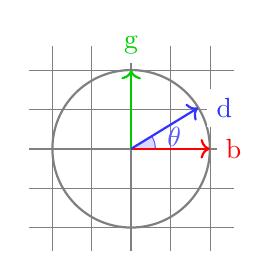
\begin{tikzpicture}
					\draw[step=.5,gray,very thin] (-1.3,-1.3) grid (1.3,1.3);
					\draw[gray, thick] (0,0) circle (1);
					\draw[gray, thick] (1.3, 0) -- (-1.3, 0);
					\draw[gray, thick] (0, 1.3) -- (0, -1.3);
					\draw[green!80!black, thick, ->] (0,0) -- (0, 1) node[above=2pt, fill=white] {g};
					\draw[blue!65!white, thick] (0.3, 0) arc (0:30:0.3) node[right=2pt] {$\theta$};
					\fill[blue!15!white] (0,0) -- (0.3, 0) arc (0:30:0.3) -- (0,0);
					\draw[red, thick, ->] (0,0) -- (1,0) node[right=2pt, fill=white] {b};
					\draw[blue!80!white, thick, ->] (0,0) -- (0.85,0.52) node[right=3pt, fill=white] {d};
				\end{tikzpicture}
			\end{minipage}
			\begin{minipage}{0.35\textwidth}
				\item Velg $\theta$ for effekt
				\begin{align*}
					\theta & = \arcsin(\frac{\sqrt{t}}{\sqrt{2}^n}) \\
					d & = \sin(\theta)g + \cos(\theta)b
				\end{align*}
			\end{minipage}
		\end{itemize}
	\end{frame}

	\begin{frame}{Grover's algoritme; IV}
		\begin{itemize}
			\item $\mathcal{O}_{f,\pm}$ er en refleksjon i planet $\mathbb{C}\{g,\ b\}$.
			\begin{align*}
				& \mathcal{O}_{f,\pm}(g) = -g \\
				& \mathcal{O}_{f,\pm}(b) = b
			\end{align*}
			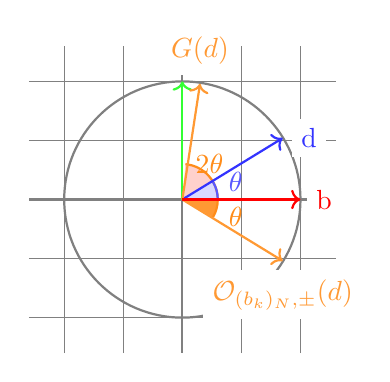
\begin{tikzpicture}[scale=1.5]
				\draw[step=.5,gray,very thin] (-1.3,-1.3) grid (1.3,1.3);
				\draw[gray, thick] (0,0) circle (1);
				\draw[gray, thick] (1.3, 0) -- (-1.3, 0);
				\draw[gray, thick] (0, 1.3) -- (0, -1.3);
				\draw[green!80!white, thick, ->] (0,0) -- (0, 1) node[above=2pt, fill=white] {g};
				\fill[red!80!orange!20!white] (0,0) -- (0.3, 0) arc (0:85:0.3) -- (0,0);
				\fill[blue!15!white] (0,0) -- (0.3, 0) arc (0:30:0.3) -- (0,0);
				\fill[orange!80!white] (0,0) -- (0.3, 0) arc (0:-30:0.3) -- (0,0);
				\draw[orange!90!white, thick] (0.3, 0) arc (0:85:0.3) node[right=0pt] {$2\theta$};
				\draw[blue!65!white, thick] (0.3, 0) arc (0:30:0.3) node[right=2pt] {$\theta$};
				\draw[orange!90!white, thick] (0.3, 0) arc (0:-30:0.3) node[right=2pt] {$\theta$};
				\draw[blue!80!white, thick, ->] (0,0) -- (0.85,0.52) node[right=3pt, fill=white] {d};
				\draw[orange!80!white, thick, ->] (0,0) -- (0.15,0.98) node[above=3.2pt, fill=white] {$G(d)$};
				\draw[orange!80!white, thick, ->] (0,0) -- (0.85,-0.52) node[below=3pt, fill=white] {$\mathcal{O}_{(b_k)_N,\pm}(d)$};
				\draw[red, thick, ->] (0,0) -- (1,0) node[right=2pt, fill=white] {b};
			\end{tikzpicture}
		\end{itemize}
	\end{frame}

\section{Kvantevandringer}

	\begin{frame}{Kvantevandringer}
		
	\end{frame}

\section{Implementasjon og tester}

	\begin{frame}{Litt om DSLer}
		
	\end{frame}

\section{Veien videre}

	\begin{frame}{Elektriske nettverk}
		
	\end{frame}

\end{document}